\section{Evaluation and Results}\label{chapt:results}

The results shown here were executed with the previously mentioned settings. The two labels \textit{optimized} and \textit{unoptimized} refer to the two different compiled kernels. The label \textit{unoptimized} means a kernel which was compiled with the default settings, the label \textit{optimized} means a kernel compiled with the custom sorted linker script. Both kernels are of version \textit{5.10.178} and were compiled with \textit{gcc-10}. The flag \textit{nokaslr} was used as an additional boot parameter.

A group of network applications was selected on which both the call stack analysis and the PMU events collection were performed. Each kernel was tested five times. PMU events were counted for 6 hours with a sampling period of 1 second, resulting in 21,600 samples per test run. Call stacks were collected for 140 seconds to avoid losing any information. A warm-up time of 10 minutes was used for each collection. Recommended settings and parameters are included from the BOLT project \cite{llvm-bolt}. Table \ref{table:numberresults} presents the geometric mean of the collected PMU events for both the optimized and unoptimized cases across all test runs.

\begin{table}[H]
    \centering
    \begin{tabular}{clccc}
        &&&&\\ [-3mm] \hline
        & \multicolumn{1}{c}{\multirow{2}{*}{PMU events and metrics}}   & \multicolumn{2}{c}{Counted values for case} & Difference \\ \cline{3-4}
        && \multicolumn{1}{c}{unoptimized} & \multicolumn{1}{c}{optimized} & in percentage  \\ \hline
        &&&&\\ [-4mm]
        \triadown & itlb\_misses.miss\_causes\_a\_walk & 1584215 & 1571755 & -0.787 \\
        \triadown & (kilo) itlb\_misses.walk\_active & 71240 & 70675 & -0.793 \\
        \triadown & itlb\_misses.walk\_completed & 726417 & 713469 & -1.782    \\
        \triadown & frontend\_retired.itlb\_miss & 359667 & 143449 & -60.116 \\
        \triadown & icache\_64b.iftag\_miss & 148360051 & 136604656 & -7.924   \\
        &&&&\\ [-3mm]
        \triaup & IPC & 2.5775 & 2.6011 & 0.916 \\
        \triadown & ITLB Stall & 2.5815 & 2.4337 & -5.725  \\
        \triadown & ITLB MPKI & 0.2036 & 0.2018 & -0.884  \\ 
        &&&&\\ [-4mm] \hline
    \end{tabular}
    \caption{Calculated geometric mean values for defined PMU events and metrics}
    \label{table:numberresults}
\end{table}
\vspace{-\baselineskip}

The first value in each row indicates whether the event or metric described should be minimized (\triadown) or maximized (\triaup). This is followed by the name of the PMU event or metric, which were defined in chapter \ref{section:events}, and the average counted value in the specified time period for the optimized and unoptimized kernel. The last column shows the calculated difference as percentage between the optimized and unoptimized values. A positive percentage indicates that the optimized value is larger than the unoptimized value, and vice versa. Additionally, the metric \textit{instructions per cycle} (IPC) has been included as reference for the general system performance.

However, the PMU events themselves are not a simple indicator of whether there is a measurable performance improvement for the application, such as faster compilation times or more searches per second. These values offer a more user-friendly way to evaluate the impact of code collocation on performance. Therefore, in addition to the PMU events, the average throughput for a network application, which is recommended for this type of application by \cite{intel_demistify}, was also tested. The throughput metric displays how much data can be sent or received during a time period. \cite[p. 22]{brendan} 

In this case, the network metrics \textit{throughput} and \textit{total bytes transferred} from the client to the server were measured for a single application on each kernel. The measurements were conducted five times, with each test run lasting for one hour. The zero-copy functionality was utilized during the measurements. In table \ref{table:throughput} displays the geometric mean of the collected measurements for both the optimized and unoptimized cases.

\begin{table}[H]
    \centering
    \begin{tabular}{clP{2cm}P{2cm}c}
        &&&&\\ [-3mm] \hline
        &\multicolumn{1}{c}{\multirow{2}{*}{Network metrics}} & \multicolumn{2}{c}{Counted values for case} & Difference \\ \cline{3-4}
        && \multicolumn{1}{c}{unoptimized} & \multicolumn{1}{c}{optimized} & in percentage  \\ \hline
        &&&&\\ [-4mm]
        \triaup & Throughput (kbit/s) & 20032754.27 & 22920552.65 & 14.415 \\
        \triaup & Total bytes (TB) & 8.198 & 9.375 & 14.357 \\
        &&&&\\ [-4mm] \hline
    \end{tabular}
    \caption{Calculated geometric mean values for throughput and total bytes transferred}
    \label{table:throughput}
\end{table}
\vspace{-\baselineskip}

Firstly, it is essential to exercise caution when interpreting the shown results, as they are specific to the test setup, the workload type and the conditions applied. Furthermore, it is important to highlight that these values have not undergone significance testing, and the results from other tests may exhibit significantly different outcomes.

In general, a positive trend can be observed in the events and metrics presented in table \ref{table:numberresults}. Although most of the events and metrics do not exhibit a significant impact from code collocation, there are three specific values that stand out: \textit{icache\_64b.iftag\_miss}, \textit{frontend\_retired.itlb\_miss}, and the \textit{ITLB Stall} metric, which exhibit reductions ranging from 5.725\% to 60.116\%. To further analyse these events and metric, their histogram distributions are to be examined.

Notably, only these two PMU events and this one metric have experienced a significant reduction impact from code collocation. This is likely due to the specific measurements performed by each event. The events, namely \textit{itlb\_misses.miss\_causes\_a\_walk}, \textit{itlb\_misses.walk\_active}, \\\textit{itlb\_misses.walk\_completed}, and along with the metric \textit{ITLB MPKI}, which incorporates the event \textit{itlb\_misses.walk\_completed}, count the amount, or cycles, of page table walks performed by executed instructions. 

This suggests that code collocation did not result in a reduction of not written back speculative executed instructions, as the workload continues to generate a similar number of page table walks even with code collocation. This situation can arise when, for instance, a cold page is to be fetched due to the branch predictor, but it is not present in the ITLB, prompting a page table walk. However, during the page table walk, it is recognized that the cold page is unnecessary, leading to the termination of the page table walk. Despite the page table walk being terminated, the page table walk caused by the fetching of the cold page is still classified as such and counted accordingly.

\newpage

In contrast icache\_64b.iftag\_miss, frontend\_retired.itlb\_miss, and the ITLB Stall metric, which incorporates the event \textit{icache\_64b.iftag\_stall}, are not as dependent on speculative execution as the other PMU events. Instead, they monitor stalls and misses that occur during instruction fetch tag lookup or count the number of retired ITLB instructions which did experience ITLB misses.

The histograms for the outstanding events can be seen in figure \ref{fig:histograms}. These histograms illustrate the events or metrics recorded per second and their frequency throughout all test runs. The data used in these histograms is based on the results from all five test runs, amounting to a total of 108000 samples per case. The mean value $\boldsymbol\mu$ and the standard deviation $\boldsymbol\sigma$ were calculated for each individual case.

The histograms provide validation for the results, as indicated in table \ref{table:numberresults}. All figures show a decrease in their values for the optimized case when compared to the unoptimized case, as illustrated in table \ref{table:numberresults}.

The presence of tails or other irregularities in the distributions, representing the influence of interfering sources, can be attributed to the test configuration. Despite prioritizing the network workload, the impact of other user space applications is still noticeable across all three figures. However, it is also evident that the adjustment of the priority of the workload had the desired effect, as a noticeable and measurable change can be observed. This influence does not appear to be as pronounced in the distribution in figure \ref{fig:histograms-stall} compared to the other distributions.

Of particular interest for interpretation is the distribution presented in figure \ref{fig:histograms-frontend} in combination with the geometric mean in table \ref{table:numberresults}. As this PMU event represents the count of retired instructions, the resulting data provides a more accurate and precise interpretation of ITLB pressure compared to PMU events which also include executed instructions, making it harder to assess the true impact of code collocation on ITLB pressure. In these test runs did not only the geometric mean decrease by approximately 60\%, but the standard deviation decreased also by around 65.86\%, from approximately 160381 to 54744.

\enlargethispage{\baselineskip}
The reduction in both the mean value and the standard deviation signifies a positive impact of code collocation. Firstly, the reduced mean value indicates fewer retired ITLB misses on average, which suggests an increase in ITLB hits. This, in turn, should lead to a decrease in ITLB stalls, as figure \ref{fig:histograms-stall} illustrates. Secondly, the reduced standard deviation implies less scattering and more consistent outcomes, indicating that the processor can rely more frequently on the pages stored in the ITLB for different operations, reducing in sum the need to fetch additional pages.

\newpage
\begin{figure}[H]
    \centering
    \begin{subfigure}{\linewidth}
        \centering
        \captionsetup{singlelinecheck=false, margin={28mm,0cm}}
        \caption{Event icache\_64b.iftag\_miss}
        \label{fig:histograms-miss}
        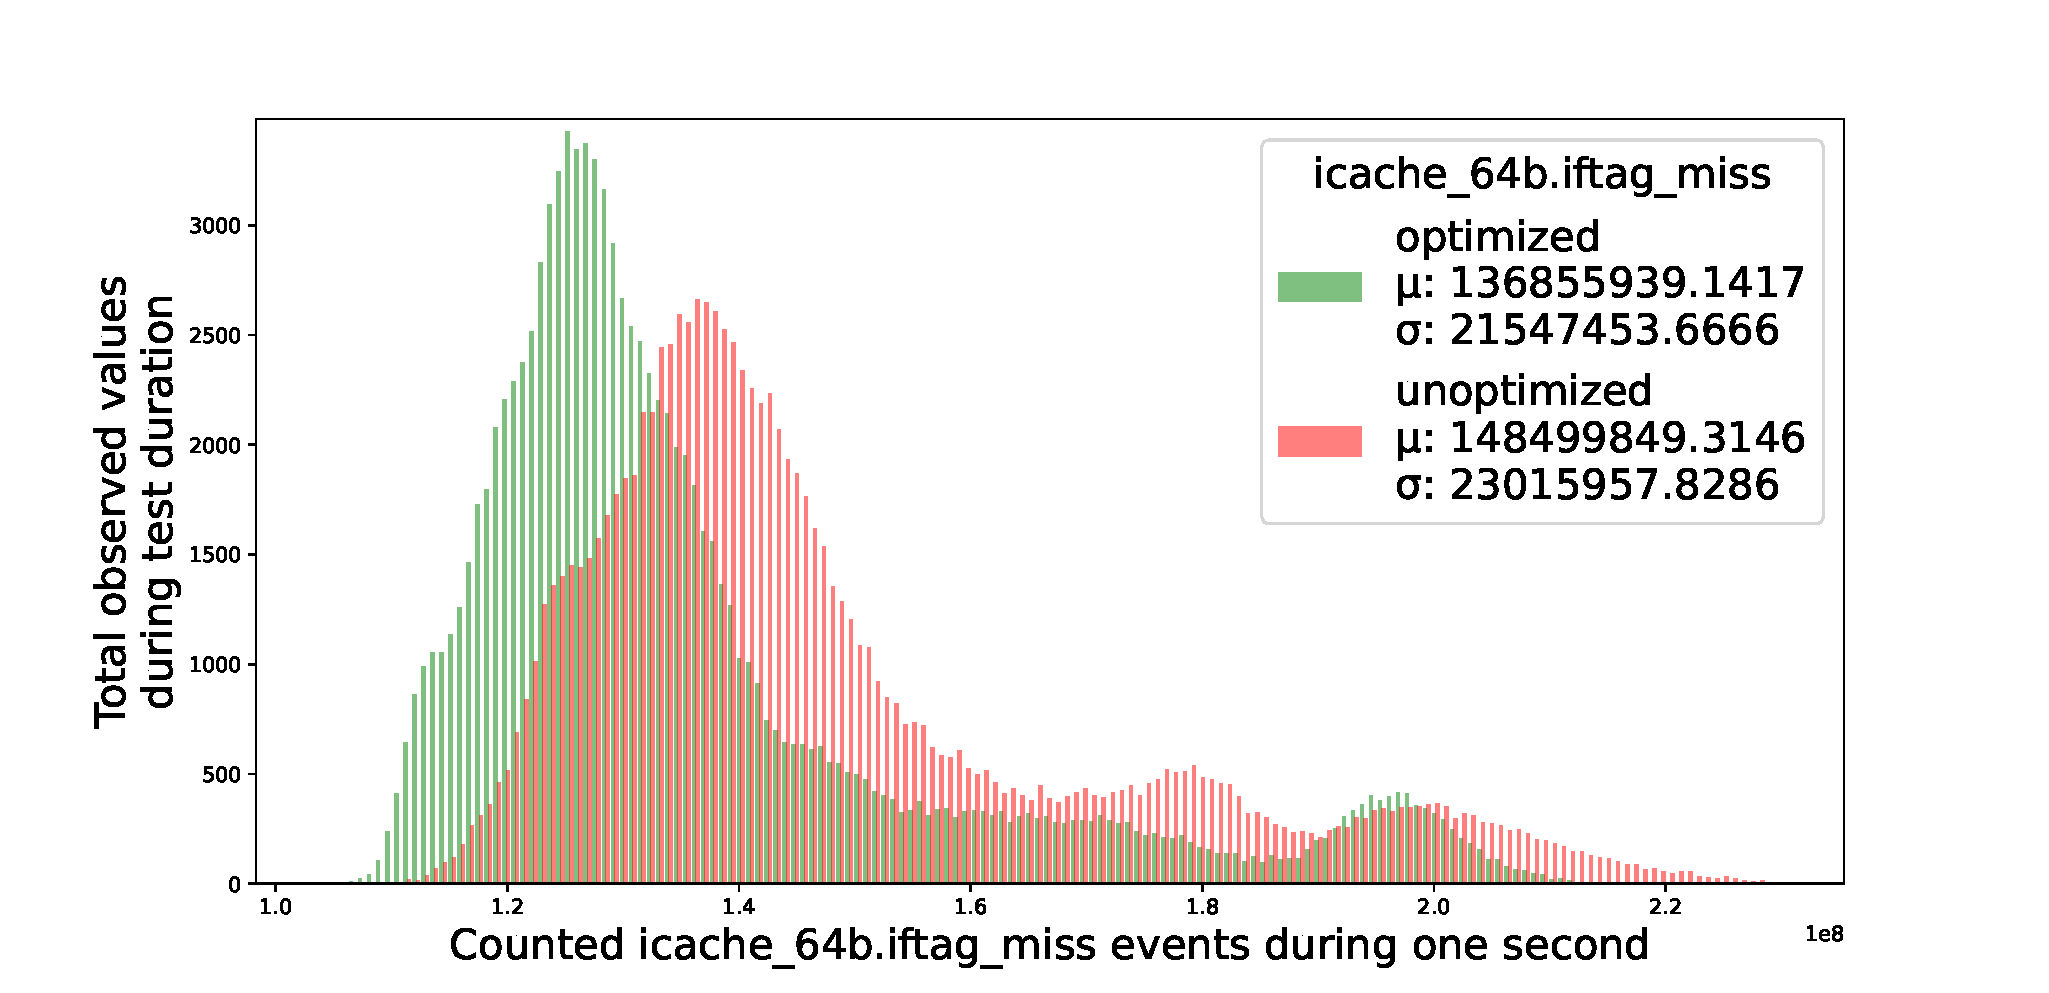
\includegraphics[width=.8\textwidth]{images/5_implementation/icache-iftag-miss.pdf}
        \vspace{.5\baselineskip}
    \end{subfigure}
    \begin{subfigure}{\linewidth}
        \centering
        \captionsetup{singlelinecheck=false, margin={29mm,0cm}}
        \caption{Metric ITLB stall}
        \label{fig:histograms-stall}
        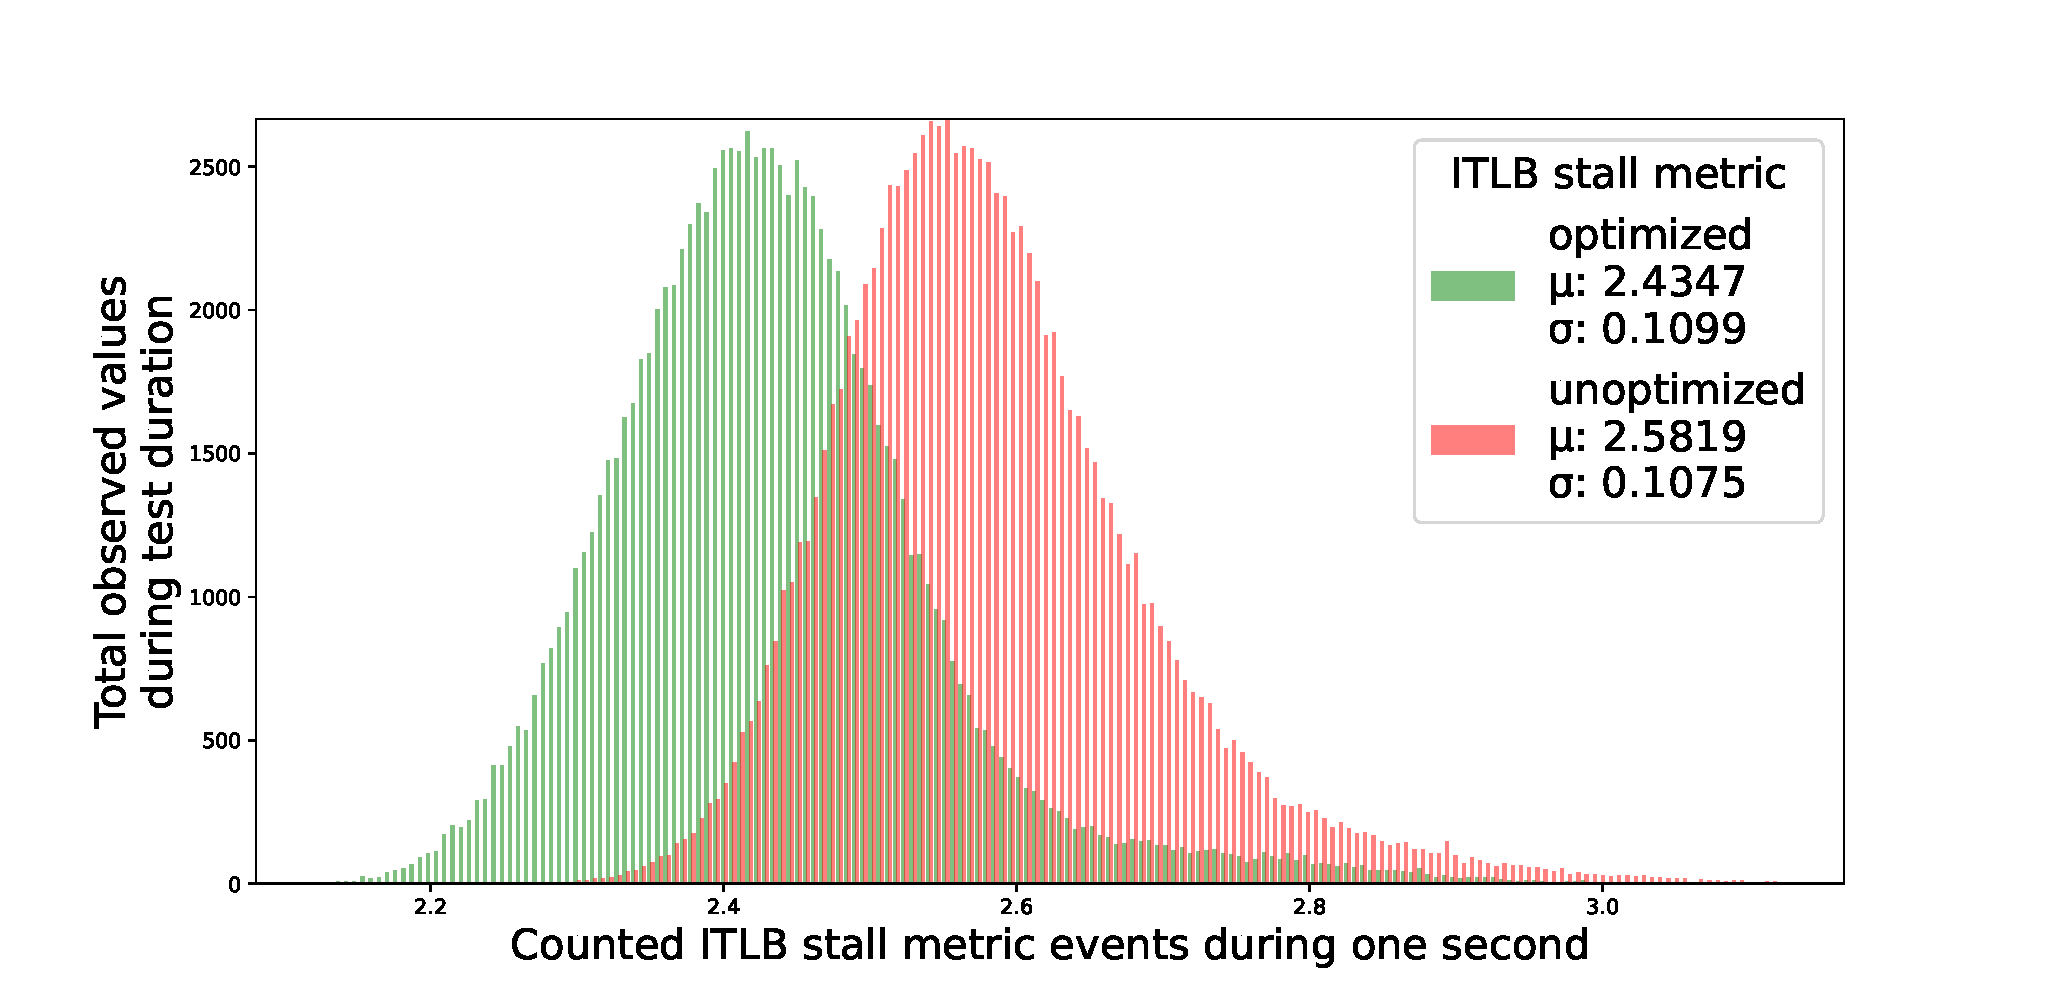
\includegraphics[width=.8\textwidth]{images/5_implementation/itlb-stall.pdf}
        \vspace{.5\baselineskip}
    \end{subfigure}
    \begin{subfigure}{\linewidth}
        \centering
        \captionsetup{singlelinecheck=false, margin={29mm,0cm}}
        \caption{Event frontend\_retired.itlb\_miss}
        \label{fig:histograms-frontend}
        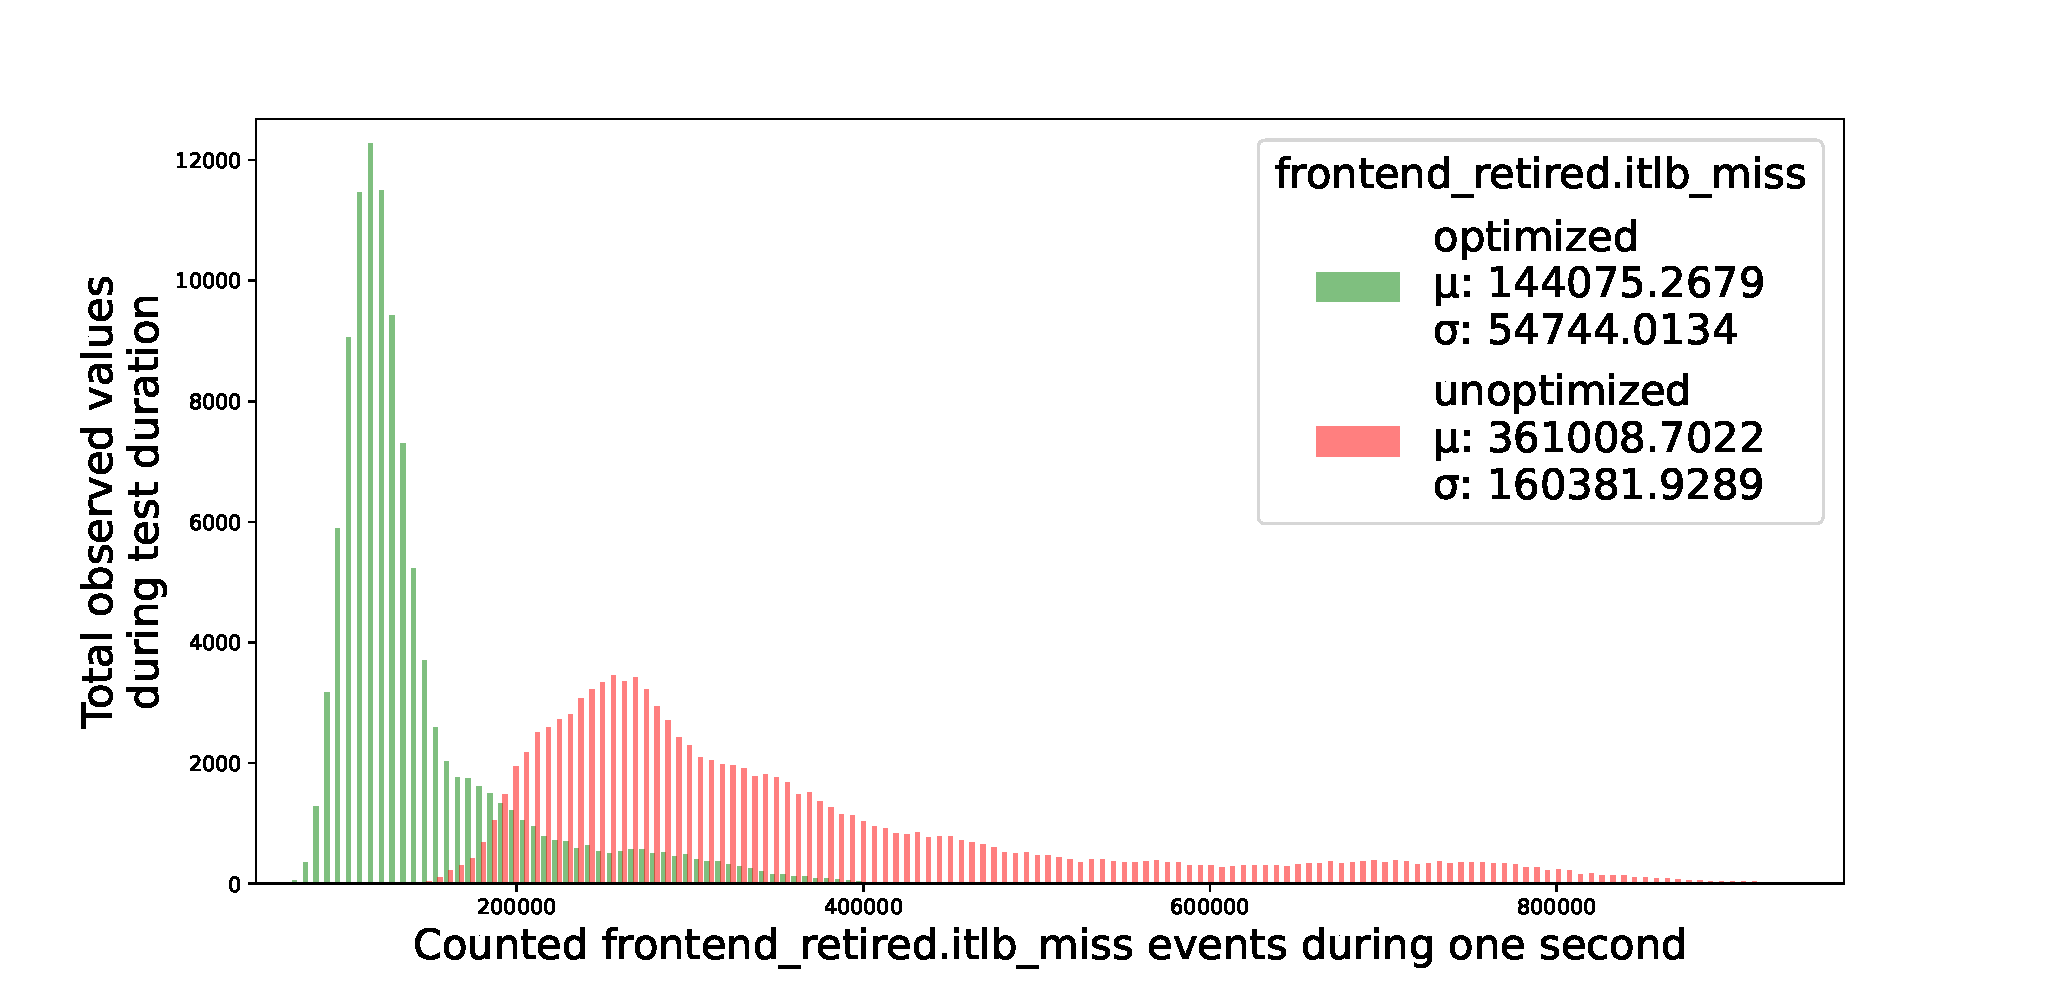
\includegraphics[width=.8\textwidth]{images/5_implementation/frontend-miss.pdf}
    \end{subfigure}
    \caption{Histograms for specific PMU events and metrics for the optimized case (green) and unoptimized case (red)}
    \label{fig:histograms}
\end{figure}
\newpage

Nevertheless, the overall decrease in all events and metrics, particularly in icache\_64b.iftag\_miss, frontend\_retired.itlb\_miss, and the ITLB stall metric, is likely the primary factor behind the observed improvements in the measured network metrics outlined in table \ref{table:throughput}, resulting in an approximate improvement of 14\% for the throughput as well as the total bytes transferred. This is also reflected by an increased IPC value of roughly 0.9\%, as illustrated in table \ref{table:numberresults}.
